\documentclass[11pt,a4paper]{article}
\usepackage[utf8]{inputenc}
\usepackage[portuguese]{babel}
\usepackage[T1]{fontenc}
\usepackage[ddmmyyyy]{datetime}
\usepackage[margin=2cm]{geometry}
\usepackage{amsfonts}
\usepackage{amsmath}
\usepackage{amssymb}
\usepackage{amsthm}
\usepackage[citestyle=authortitle]{biblatex}
\usepackage{csquotes}
\usepackage{graphicx}
\usepackage{mathtools}
\usepackage{thmtools}
\usepackage{titling}
\usepackage{xcolor}
\usepackage{enumitem}
\usepackage[unicode]{hyperref}

\pdfsuppressptexinfo=7

\graphicspath{{e-folio/e-folio-a/imagem}}
\addbibresource{bibliografia.bib}

% Ambientes de provas e demonstrações
\newtheorem{proposition}{Proposição}[section]
\renewcommand\qedsymbol{\textbf{q.e.d.}}

% Dados
\author{Carlos Augusto Gonçalves Collaço e Pinto Machado}
\newcommand{\numeroEstudante}{2200909}
\newcommand{\UC}{Álgebra Linear I}
\newcommand{\codigoUC}{21002}
\newcommand{\docentes}{Wolfram Bentz}
\newcommand{\curso}{Licenciatura em Matemática e Aplicações}
\newcommand{\turma}{5}
\newcommand{\anoLectivo}{2023-2024}
\date{\today}

\pagenumbering{arabic}

\hypersetup{
	pdfsubject={\UC},
	pdftitle={E-fólio A - \numeroEstudante},
	pdfauthor={Carlos Pinto Machado},
	pdfproducer={},
	pdfcreator={}
}

\makeindex

\newcommand{\grupo}{
	\addtocounter{section}{1}
	\setcounter{subsection}{0}
	\setcounter{proposition}{0}
	\section*{\Roman{section}.}
	\phantomsection
	\addcontentsline{toc}{section}{Grupo \arabic{section}}
}

\newcommand{\exercicio}{
	\addtocounter{subsection}{1}
	\subsection*{\arabic{subsection}}
	\addcontentsline{toc}{subsection}{Exercício \arabic{subsection}}
}


\begin{document}

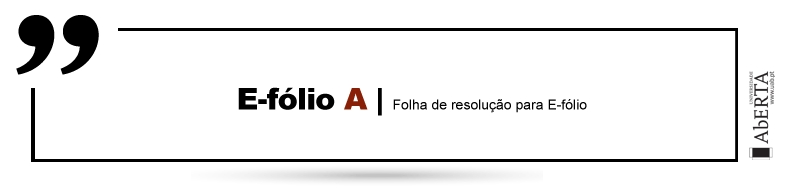
\includegraphics[width=\textwidth]{e-folio-a.jpg}

\paragraph{\textbf{UNIDADE CURRICULAR:}} \UC

\paragraph{\textbf{CÓDIGO:}} \codigoUC

\paragraph{\textbf{DOCENTE:}} \docentes

\paragraph{\textbf{NOME:}} \theauthor

\paragraph{\textbf{N.º DE ESTUDANTE:}} \numeroEstudante

\paragraph{\textbf{CURSO:}} \curso

\paragraph{\textbf{DATA DE ENTREGA:}} \thedate


\clearpage

\grupo{}

\exercicio{}

\paragraph{\underline{Resposta}}

\paragraph{}É a opção d). $CB$ é invertível.

\paragraph{\underline{Justificação}}

\begin{align*}
	\intertext{Tem-se que as matrizes $A$, $B$ e $C$ são definidas por}
	A =
	\begin{bmatrix*}[r]
		2  & 3\\
		2  & 0\\
		-3 & 1
	\end{bmatrix*}
	\in
	\mathcal{M}_{3 \times 2}(\mathbb{K})
	,\;
	B =
	\begin{bmatrix*}[r]
		-3\\
		1
	\end{bmatrix*}
	\in
	\mathcal{M}_{2 \times 1}(\mathbb{K})
	 \text{ e }
	C =
	\begin{bmatrix*}[r]
		1  & 2
	\end{bmatrix*}
	\in
	\mathcal{M}_{1 \times 2}(\mathbb{K})
	.
\end{align*}

\vspace{0.25cm}

\begin{proposition}[negação da opção 1.a]\label{prop:i-1-a}
	$AB$ é definido.
\end{proposition}

\vspace{0.25cm}

\begin{proof}
	\; \\
	Pela definição da matriz produto
	\footcite[pág. 12, Definição 1.18: matriz produto]{Cabral2012},
	esta só é definida se o número de colunas do
	operando à esquerda for igual ao número de linhas do operando à
	direita. Como
	$A$ tem o mesmo número de colunas que o número de linhas de $B$,
	então $AB$ é definido.\\
\end{proof}

\begin{proposition}[negação da opção 1.b]\label{prop:i-1-b}
	$AC$ não é definido.
\end{proposition}

\vspace{0.25cm}

\begin{proof}
	\; \\
	Pela definição da matriz produto
	\footcite[pág. 12, Definição 1.18: matriz produto]{Cabral2012},
	esta só é definida se o número de colunas do
	operando à esquerda for igual ao número de linhas do operando à
	direita. Como
	$A$ tem um número de colunas diferente do número de linhas de $C$,
	então $AC$ não é definido.\\
\end{proof}

\begin{proposition}[negação da opção 1.c]\label{prop:i-1-c}
	$(BC)^2$ não é invertível.
\end{proposition}

\vspace{0.25cm}

\begin{proof}
	\; \\
	Pela definição da matriz produto
	\footcite[pág. 12, Definição 1.18: matriz produto]{Cabral2012},
	tem-se que:
	\begin{align*}
		BC &=
		\begin{bmatrix*}[r]
			-3\\
			1
		\end{bmatrix*}
		\begin{bmatrix*}[r]
			1  & 2
		\end{bmatrix*}
		=
		\begin{bmatrix*}[r]
			-3  & -6\\
			1  & 2\\
		\end{bmatrix*}
		\intertext{
			Dado que as linhas de $BC$ não são linearmente
			independentes, e que a operação $l_i + \beta l_j$
			não tem impacto no determinante
			\footcite[pág. 138, Proposição 3.19, alínea 3.]{Cabral2012},
			tem-se que:}
			BC&
		\overset{l_1 + 3 l_2}{\longrightarrow}
		\begin{bmatrix*}[r]
			0  & 0\\
			1  & 2\\
		\end{bmatrix*}
		\implies \det(BC) = 0
		\intertext{
			Dado que o determinante da matriz produto é igual ao produto dos
			determinantes do operandos
			\footcite[pág. 145, Proposição 3.24]{Cabral2012}, tem-se que:
		}
		\det((BC)^2) = (\det(BC))^2 = 0
	\end{align*}
	Dado que a matriz só é invertível, se o determinante não for nulo
	\footcite[pág. 144, Proposição 3.23]{Cabral2012}, concluímos que
	$(BC)^2$ não é invertível.\\
\end{proof}

\clearpage
\begin{proposition}[opção 1.d]\label{prop:i-1-d}
	$CB$ é invertível.
\end{proposition}

\vspace{0.25cm}

\begin{proof}
	Pela definição da matriz produto
	\footcite[pág. 12, Definição 1.18: matriz produto]{Cabral2012},
	tem-se que:
	\begin{align*}
		CB =
		\begin{bmatrix*}
			1 & 2
		\end{bmatrix*}
		\begin{bmatrix*}[r]
			-3\\
			1
		\end{bmatrix*}
		=
		\begin{bmatrix}
			-1
		\end{bmatrix} \implies \det (CB) = -1 \neq 0
	\end{align*}
	Dado que a matriz só é invertível, se o determinante não for nulo
	\footcite[pág. 144, Proposição 3.23]{Cabral2012}, concluímos que
	$CB$ é invertível.
\end{proof}

\clearpage


\exercicio{}

\paragraph{\underline{Resposta}}

\paragraph{} É a opção b). $\det(-A(B + C)^{-1}) = 3i$.


\paragraph{\underline{Justificação}}


\paragraph{}Sejam $A, B, C \in \mathcal{M}_{4 \times 4}(\mathbb{C})$ tais que
$\det A = 3$, e $\det(B + C) = i$.

\vspace{0.25cm}

\begin{proposition}[negação da opção a]\label{prop:i-2-a}
	Não existe elementos para calcular $\det(A + B + C)$, pelo que não é
	possível afirmar que $\det(A + B + C) = 3 + i$.
\end{proposition}

\begin{proof}\;\\
	Consideremos que
	\begin{align*}
		&\exists A, B \in \mathcal{M}_{n \times n}(\mathbb{K}), \; n \geq 2:
		\;
		\det(A+B) \neq \det A + \det B
		\intertext{Exemplo:}
		&\det(I_n + 2I_n) = 3^n \neq 1 + 2^n = \det I_n + \det(2I_n)
	\end{align*}
	Portanto não existe a implicação de que
	$\det A + \det(B + C) = \det(A + B + C)$,
	ou informação para poder determinar
	$\det(A + B + C)$.
	Pelo que a proposição \ref{prop:i-2-a} está demonstrada e a opção a) não
	está correcta, ou antes não pode ser deduzida dos
	factos conhecidos.\\
\end{proof}


\begin{proposition}[opção b]\label{prop:i-2-b}
	$\det(-A(B + C)^{-1}) = 3i$
\end{proposition}

\vspace{0.25cm}

\begin{proof}[Cálculo do determinante da Proposição \ref{prop:i-2-b}]
	\begin{align*}
		\det(-A(B + C)^{-1})
			   = (- \det A)  \cdot (\det(B + C))^{-1}
			   = -\frac{3}{i}
			   = -\frac{3}{i} \cdot \frac{i}{i}
			   = 3i
	\end{align*}
	Pelo que a proposicão \ref{prop:i-2-b} é verdadeira e a opção b) está correcta.\\
\end{proof}


\begin{proposition}[negação da opção c]\label{prop:i-2-c}
	Não existe elementos para calcular $\det(A^2 BC)$, pelo que não é
	possível afirmar que $\det(A^2 BC) = 9i$.
\end{proposition}

\vspace{0.25cm}

\begin{proof}
	\; \\
	Dado que desconhecemos $\det B$ e $\det C$ ou  $\det(BC)$, não existe informação
	suficiente determinar $\det(A^2BC)$.
	Pelo que a proposição \ref{prop:i-2-c} está demonstrada e a opção c) não
	está correcta, ou antes não pode ser deduzida dos
	factos conhecidos.\\
\end{proof}

\begin{proposition}[negação da opção d]\label{prop:i-2-d}
	$\det(-(B + C)A^{-1}) \neq \frac{i}{3}$
\end{proposition}

\vspace{0.25cm}

\begin{proof}[Cálculo do determinante da Proposição \ref{prop:i-2-d}]
	\begin{align*}
		\det(-(B + C)A^{-1})
			   = (-\det(B + C))  \cdot (\det A)^{-1}
			   = -\frac{i}{3} \neq \frac{i}{3}
	\end{align*}
	Pelo que está demonstrada a Proposição \ref{prop:i-2-d} e que a opção d)
	não está correcta.\\
\end{proof}




\clearpage
\grupo{}

\begin{align*}
	A &=
	\begin{bmatrix*}[r]
		2 & 1 & 0 & 3 & 0\\
		3 & -1 & 1 & 4 & 0\\
		0 & 0 & 2 & 1 & 1\\
		0 & 0 & 3 & 0 & 1\\
		0 & 0 & 1 & 0 & -2
	\end{bmatrix*},
	\quad
	b =
	\begin{bmatrix*}[r]
		0\\
		1\\
		2\\
		r_3\\
		0
	\end{bmatrix*}\\
	r_3 &= 909
\end{align*}


\begin{enumerate}[label=\alph*.]
	\item $\det A = ?$
	\item\hfill
		\begin{proposition}
			A equação $AX = b$ tem uma solução única
			$X = (x_1, x_2, x_3, x_4, x_5)^T$.
		\end{proposition}
		\begin{align*}
			x_4 = ?
		\end{align*}
\end{enumerate}

\clearpage
\grupo{}

\begin{equation}
	\begin{cases}
		ax + cy = 1\\
		-ax - 2y -az = -3\\
		2y + 2az = 2c
	\end{cases}
\end{equation}

\begin{align*}
	\intertext{O sistema na forma matricial é equivalente a}
	\begin{bmatrix*}[r]
		a  & c  & 0\\
		-a & -2 & -a\\
		0  & 2  & 2a
	\end{bmatrix*}
	&\begin{bmatrix*}[r]
		x\\
		y\\
		z
	\end{bmatrix*}
	=
	\begin{bmatrix*}[r]
		1\\
		-3\\
		2c
	\end{bmatrix*}
	\intertext{Aplicando o método }
	\begin{bmatrix*}[r]
		a  & c  & 0  & \vline & 1 \\
		-a & -2 & -a & \vline & -3\\
		0  & 2  & 2a & \vline & 2c
	\end{bmatrix*}
	&
	\begin{matrix}
		l_2 + l_1\\
		\frac{1}{2}l_3\\
		\longrightarrow
	\end{matrix}
	\begin{bmatrix*}[r]
		a & c    & 0  & \vline & 1 \\
		0 & -2+c & -a & \vline & -2\\
		0 & 1    & a  & \vline & c
	\end{bmatrix*}
	\begin{matrix}
		l_2 \leftrightarrow l_3\\
		\longrightarrow
	\end{matrix}
	\begin{bmatrix*}[r]
		a & c    & 0  & \vline & 1 \\
		0 & 1    & a  & \vline & c\\
		0 & -2+c & -a & \vline & -2
	\end{bmatrix*}\\
	\begin{matrix}
		l_3 + (2 - c)l_2\\
		\longrightarrow
	\end{matrix}
	\begin{bmatrix*}[r]
		a & c & 0  & \vline & 1 \\
		0 & 1 & a  & \vline & c\\
		0 & 0 & a - ac & \vline & -2 +2c - c^2
	\end{bmatrix*}&
	\intertext{Aplicando o método }
	\det A =
	\det \begin{bmatrix*}[r]
		a  & c  & 0\\
		-a & -2 & -a\\
		0  & 2  & 2a
	\end{bmatrix*}
	&
	\begin{matrix}
		\text{Lapl.}\\
		=\\
		c_1
	\end{matrix}
	a
	\det \begin{bmatrix*}[r]
		-2 & -a\\
		2  & 2a
	\end{bmatrix*}
	-
	(-a)
	\det \begin{bmatrix*}[r]
		c  & 0\\
		2  & 2a
	\end{bmatrix*}\\
	&=
	a\left(
	\det \begin{bmatrix*}[r]
		-2 & -a\\
		2  & 2a
	\end{bmatrix*}
	+
	\det \begin{bmatrix*}[r]
		c  & 0\\
		2  & 2a
	\end{bmatrix*}\right)\\
	&=
	a\left[
		-2 \cdot 2a - 2 \cdot (-a) +
		c \cdot 2a\right]\\
	&= 2a^2(-2 + 1 + c) = 2a^2(c - 1)
	\intertext{O sistema é indeterminado ou impossível para}
	0&= 2a^2(c - 1)\\
	\iff a &= 0 \quad \lor \quad c = 1
\end{align*}

\begin{align*}
	\begin{bmatrix*}[r]
		1 & 0 & 0 & \frac{- c^{2} + 3 c - 1}{a c - a}\\
		0 & 1 & 0 & \frac{c - 2}{c - 1}\\
		0 & 0 & 1 & \frac{c^{2} - 2 c + 2}{a c - a}
	\end{bmatrix*}
\end{align*}


\grupo{}

\begin{align*}
	A =
	\begin{bmatrix*}[r]
		1  & i  & 0\\
		-i & -1 & 0\\
		0  & 0  & 3
	\end{bmatrix*}
	\in \mathcal{M}_{3 \times 3} (\mathbb{C})
\end{align*}

\begin{align*}
	\intertext{Pretende-se determinar todas as matrizes em
	$\mathcal{M}_{3 \times 3}(\mathbb{C})$ que comutam com $A$, ou seja:}
	X &\in \mathcal{M}_{3 \times 3}(\mathbb{C}): XA = AX
	\intertext{Pelo que vamos definir uma dada matriz $X$ e calcular $XA$ e $AX$:}
	X
	&=
	\begin{bmatrix*}[r]
		U\\
		V\\
		W
	\end{bmatrix*}
	=
	\begin{bmatrix*}[r]
		u_1 & u_2 & u_3 \\
		v_1 & v_2 & v_3 \\
		w_1 & w_2 & w_3
	\end{bmatrix*}\\
	XA
	&=
	\begin{bmatrix*}[r]
		u_1 & u_2 & u_3 \\
		v_1 & v_2 & v_3 \\
		w_1 & w_2 & w_3
	\end{bmatrix*}
	\begin{bmatrix*}[r]
		1  & i  & 0\\
		-i & -1 & 0\\
		0  & 0  & 3
	\end{bmatrix*}
	=
	\begin{bmatrix*}[r]
		u_1 - iu_2 & iu_1 - u_2 & 3u_3 \\
		v_1 - iv_2 & iv_1 - v_2 & 3v_3 \\
		w_1 - iw_2 & iw_1 - w_2 & 3w_3
	\end{bmatrix*}\\
	AX
	&=
	\begin{bmatrix*}[r]
		1  & i  & 0\\
		-i & -1 & 0\\
		0  & 0  & 3
	\end{bmatrix*}
	\begin{bmatrix*}[r]
		u_1 & u_2 & u_3 \\
		v_1 & v_2 & v_3 \\
		w_1 & w_2 & w_3
	\end{bmatrix*}
	=
	\begin{bmatrix*}[r]
		u_1 + iv1   & u_2 + iv2   & u_3 + iv3 \\
		-iu_1 - v_1 & -iu_2 - v_2 & -iu_3 - v_3\\
		3w_1        & 3w_2        & 3w_3
	\end{bmatrix*}
	\intertext{Dado que $XA = AX \iff XA - AX = 0_{3 \times 3}$,
		vamos determinar $XA - AX$:}
	XA - AX
	&= 
	\begin{bmatrix*}[r]
		u_1 + iu_2 & iu_1 - u_2 & 3u_3 \\
		v_1 + iv_2 & iv_1 - v_2 & 3v_3 \\
		w_1 + iw_2 & iw_1 - w_2 & 3w_3
	\end{bmatrix*}
	-
	\begin{bmatrix*}[r]
		u_1 + iv1   & u_2 + iv2   & u_3 + iv3 \\
		-iu_1 - v_1 & -iu_2 - v_2 & -iu_3 - v_3\\
		3w_1        & 3w_2        & 3w_3
	\end{bmatrix*}\\
	&=
	\begin{bmatrix*}[r]
		iu_2 - iv_1        & iu_1 - 2u_2 - iv_2 & 2u_3 -iv_3 \\
		2v_1 + iv_2 + iu_1 & iv_1 + iu_2        & 4v_3 + iu_3 \\
		-2w_1 + iw_2       & iw_1 - 4w_2        & 0
	\end{bmatrix*}
\end{align*}


\grupo{}

\paragraph{} 


\begin{align*}
	\intertext{Sejam $n\geq 1$, $A \in \mathcal{M}_{n \times n}(\mathbb{R})$,
		tal que $A$ tem a forma}
	A =
	\begin{bmatrix*}[r]
		0 & 0 & \ldots & 0 & 0 & a_1\\
		0 & 0 & \ldots & 0 & a_2 & *\\
		0 & 0 & \ldots & a_3 & * & *\\
		\vdots & \vdots & \iddots & \vdots & \vdots & \vdots\\
		0 & a_{n -1} & \ldots & * & * & *\\
		a_n & * & \ldots & * & * & *
	\end{bmatrix*}
	\intertext{onde $a_1, a_2, \ldots, a_n \in \mathbb{R}$ e os * representam
		também valores arbitrários de $\mathbb{R}$, que podem ou não ser
	distintos.}
\end{align*}

\begin{proposition}
	$\det A = (-1)^p \prod_{k=1}^{n} a_k$, com $p = \lfloor
	\frac{n}{2}\rfloor$.
\end{proposition}

\begin{proof}\; \\
	Pode-se observar que a matriz $A$ é equivalente por linhas com uma
	matriz triangular superior $B$, por sucessivas transformações lineares de
	$l_i \leftrightarrow l_{n - i}$, com $i = 1, \ldots, \lfloor \frac{n}{2}\rfloor$. Pela Proposição 3.15 da
	bibliografia\footcite[pág. 135, Proposição 3.15]{Cabral2012}, tem-se que
	$\det B = \prod_{k=1}^{n} b_k$, o produto dos elementos da diagonal principal de $B$. A
	partir da Proposição 3.19, alínea 1., da bibliografia
	\footcite[pág. 138, Proposição 3.19, alínea 1.]{Cabral2012}, tem-se que
	cada mudança de linhas o determinante é igual ao seu simétrico.
	Deste modo, com $p = \lfloor\frac{n}{2}\rfloor$ transformações lineares
	desse tipo, podemos concluir que $\det A = (-1)^p \prod_{k=1}^{n}
	a_k$.\\
\end{proof}



\clearpage
\nocite{Cabral2012}
\printbibliography[heading=bibintoc,title={Bibliografia}]

\end{document}
